\documentclass[conference]{IEEEtran}

% --- Encoding and fonts ---
\usepackage[T1]{fontenc}
\usepackage[utf8]{inputenc}
\usepackage{lmodern}
\usepackage{microtype}

% --- URLs ---
\usepackage{url}
\usepackage{xurl}

% --- Math ---
\usepackage{amsmath}
\usepackage{amssymb}

% --- Tables ---
\usepackage{tabularx}
\usepackage{booktabs}

% --- Graphics ---
\usepackage{graphicx}
\usepackage{tikz}
\usetikzlibrary{arrows.meta, positioning, calc}

% --- Code listings (JSON in Appendix A) ---
\usepackage{listings}
\lstdefinestyle{janusjson}{%
  basicstyle=\ttfamily\footnotesize,
  showstringspaces=false,
  keepspaces=true,
  breaklines=false,
  breakatwhitespace=true,
  columns=fullflexible,
  upquote=true,
  numbers=none,
  frame=single,
  rulecolor=\color{black!18},
  backgroundcolor=\color{black!01},
  framerule=0.3pt,
  framesep=0.7em,
  aboveskip=1.1em,
  belowskip=1.1em,
  xleftmargin=0.5em,
  xrightmargin=0.5em,
}
\lstdefinelanguage{json}{}
\lstset{language=json,style=janusjson}

\title{The Missing Decision Layer: Structural Failure in Information Systems and the Case for a Minimal Governance Kernel\\
\large Version 1.1 Candidate}

\author{%
  \IEEEauthorblockN{Martín Nicolás Sánchez Morales}\\
  \IEEEauthorblockA{Janus Governance Project\\
  Buenos Aires, Argentina\\
  ORCID: \url{https://orcid.org/0009-0000-4963-8847}\\
  \url{https://janusgovernance.org}}%
}

\begin{document}

\maketitle

\begin{abstract}
This paper proposes that information systems often record state changes and the
operations that produced them without preserving, as a first-class component,
the human decision associated with outcomes that require explicit accountability.
We call this proposed structural condition the \emph{governance gap}. The claim
is a paper thesis and an optional framework profile; Janus Core Lite requires a
\texttt{HUMAN\_DECISION} only when explicit human accountability is required.

This paper presents a retrospective longitudinal practitioner study based on
professional experience and corroborating publicly available sources. No
confidential administrative records or identifiable personal data are
reproduced. The five contexts span approximately four decades; each section
distinguishes publicly verifiable records, de-identified practitioner
observations, retrospective practitioner recollection, and academic inference.

This paper presents that longitudinal account, documents recurring failure modes,
and introduces a decision-binding profile built on the Janus Core and Framework
models~\cite{sanchez_core,sanchez_framework}. The profile is proposed for
AI-assisted development contexts; it does not add requirements to Janus Core.
\end{abstract}

\begin{IEEEkeywords}
decision layer, governance gap, governance kernel, structural systems failure, accountability, reconstructibility, AI governance, information systems design, append-only records, evidence model, public administration
\end{IEEEkeywords}

\section*{Independence and Confidentiality Statement}

This is independent research by the author. It does not represent an official
position, endorsement, or institutional assessment by the Direcci\'on General
de Cultura y Educaci\'on, any district-level authority, or any other public
body. Janus was developed independently by the author, informed in part by
longitudinal professional experience across multiple institutional and
technical contexts.

\section{Structural Failure in Information Systems}

Many information systems emphasize state and operations. A state change may be
recorded and the operation logged while the human authorization relevant to an
accountable outcome remains external to the system.

The paper treats this as a possible architectural failure rather than merely a
logging defect. The scope is limited to decisions for which explicit human
accountability is required.

The paper hypothesizes that this absence can impair reconstruction when a state
is contested in an audit, legal challenge, personnel transition, or system
failure. The degree and consequence of that impairment depend on the system,
the available records, and the applicable accountability requirements.

The author's professional experience includes legacy data environments,
spreadsheet-based administration, relational databases, script-driven
workflows, and AI-assisted development. Similar observations across these
contexts motivate a technology-independent hypothesis; they do not establish
that the same failure is present across implementations generally.

\subsection{Contributions}

This paper makes three primary contributions:

\begin{enumerate}
  \item It advances the missing decision layer as a structural-failure
  hypothesis in information system design, distinct from implementation quality
  or logging discipline.
  \item It presents longitudinal practitioner testimony that motivates a
  hypothesis across public administration, education governance, software
  development, and AI-assisted production.
  \item It documents a decision-binding framework profile built on the Janus
  Core concepts of evidence, canonical logs, and human authority.
\end{enumerate}

\section{Why Systems Are Not Reconstructible}

For the optional decision-binding profile proposed by this paper, reconstructing
accountable state from authorized decisions requires the following conditions:

\begin{enumerate}
  \item Every state change in the declared profile scope is traceable to an operation.
  \item Every accountable operation in that scope is traceable to a decision.
  \item Every decision must be attributable to an accountable actor.
  \item The record must be append-only and internally auditable.
\end{enumerate}

This paper does not estimate how frequently existing systems satisfy these
conditions. That question requires a separate empirical study.

When condition~2 fails, the paper describes a possible gap between what the
system records and what authorized the change. In the cases recalled by the
author, reconstruction then depended on informal memory, physical archives, or
negotiation between conflicting records. Such mechanisms may be difficult to
transfer and may be lost when the people who hold the relevant knowledge are no
longer available.

The paper's structural hypothesis is that a system without a decision layer may
record what changed without preserving the accountable authorization chain.

\subsection{The AI Amplification Problem}

AI-assisted development does not necessarily introduce this proposed failure,
but it may amplify its effects.

In human-paced development, the governance gap accumulates at human speed. Informal compensatory mechanisms --- institutional memory, experienced colleagues, organizational documentation --- partially close it. These mechanisms are imperfect, but they operate within the constraints of human time and human process.

In AI-assisted development, three conditions change simultaneously. First, velocity: an AI agent can generate, modify, and deploy artifacts across multiple files and systems within a single session. The governance gap accumulates at machine speed. Second, memory: an AI agent carries no institutional memory between sessions. It operates on the current state of data. If the decision record does not exist in the system, the agent cannot reconstruct it --- outputs may be technically coherent with the current state but institutionally incoherent with the decisions that produced that state. Third, attribution: when an AI agent modifies a system artifact, the authorization chain --- who decided this, why, and with what authority --- becomes structurally more complex and, without a governance layer, invisible.

Whether informal compensatory mechanisms remain adequate at AI-assisted
development velocity is an empirical question. This paper proposes that the
risk increases when authorization records are absent.

\section{Retrospective Longitudinal Practitioner Study}

The proposed failure pattern is grounded in five contexts recalled across
approximately four decades of professional experience. The cases are
illustrative and hypothesis-generating; they do not constitute a representative
sample. Public sources support only the specific historical and technical facts
cited below. Other case descriptions are practitioner testimony or retrospective
recollection, and the cross-case interpretation is academic inference.

\subsection{Reported Recurrent Pattern}

Across the cases recalled by the author, the following sequence recurred:

\begin{enumerate}
  \item A system is built to manage data.
  \item Humans use it to make decisions over that data.
  \item The data is recorded; the decisions are not.
  \item When data is contested, the decision record does not exist.
  \item Resolution depends on informal memory, physical archives, or negotiation between conflicting systems.
\end{enumerate}

The recurrence reported across the author's longitudinal professional experience
suggests a persistent governance pattern and motivates a structural hypothesis;
it does not, by itself, establish a universal invariant.

The paper interprets this as a governance-architecture pattern rather than a
technology-specific defect~\cite{trist1951}. That interpretation remains a
research hypothesis to be tested against independently documented cases.

\subsection{National-Scale Administration: Practitioner Account (2000--2002)}

The author reports professional participation in a technical-assistance context
in Argentina against a 2000--2001 background recalled as a period of emergency,
followed by implementation work. That background is retrospective practitioner
recollection, not a fact attributed to Decree 1369/2001. Decree 1369/2001, dated
29 October 2001 and published on 31 October 2001, is cited solely to establish
the official denomination of the ministry in 2001~\cite{decree1369}. The
Programa Jefes de Hogar was created in 2002 by Decree
565/2002~\cite{decree565}. The account of technical work is practitioner
testimony. This revision does not repeat unsupported beneficiary or throughput
figures and does not attribute the engagement to a specific sponsor.

\subsection{Municipal and Provincial Administration}

The author reports professional experience in public administration and
technical-administrative systems across subsequent municipal and provincial
contexts. The recollection is that some systems preserved operational state
without preserving the associated decision rationale as a first-class record.
An exact office, title, employment status, or individual administrative action
is unnecessary to the academic claim; those details are omitted here.

At provincial scale, the relevant public context is education administration in
Buenos Aires Province. The case in Section~IV is de-identified and limited to a
structural observation; it does not assess any identified institution or
platform.

The recurrence described by the author motivates comparative research. It is not
presented here as a measured prevalence claim about information systems generally.

\section{De-identified Case: Public Education Administration}

The author presents a district-level public education administration office in
Buenos Aires Province as a retrospective practitioner case. The account is based
on professional experience; no confidential administrative record, identifiable
personal data, internal procedure, access mechanism, named platform defect, or
specific vulnerability is reproduced.

\subsection{Structural Observation}

The observation relevant to this paper is narrow: operational records and
authorization rationale can be maintained in separate places, so a later reader
may be able to reconstruct a change without reconstructing the accountable
decision associated with it. The paper does not claim that this condition is
unique to, universal within, or officially established for provincial public
education administration.

\subsection{Academic Inference}

The case motivates the hypothesis that a governance layer may complement an
existing administrative system by preserving accountable decisions and their
declared objects. That inference does not identify a particular technical
architecture, prescribe remediation for an institution, or evaluate any public
body. Independent empirical work would be required to assess prevalence,
causation, and operational impact.

\section{Experimental Case: The 3D Dice}

\subsection{Context}

The author reports that a Three.js 3D dice component was developed as part of a
trivia module for an educational platform. Public git history in the repository
\texttt{lluviadeideas-juegosdidacticos/trivias} provides documentary evidence for
five of the six timeline entries discussed in v1.0. The relevant implementation
path is \texttt{src/trivia/HomeScreen.js}, not \texttt{dice3d.js}.

\subsection{The Problem and Its Resolution}

The component exhibited the following structural condition: the rotation engine calculated face positions in a coordinate space defined by the rendering engine; visual output was determined in a separate representation space. The value produced by the calculation logic did not match the face presented to the user.

Two representations of the same state in disagreement, with no system-native mechanism to determine which was authoritative. This is structurally identical to decision invisibility: a system records a state change but the record contains no information about which representation is correct or what authorized the transition to that state.

The resolution was instrumentation: console telemetry was used to observe actual runtime state at the exact point of discrepancy. Variables were rewritten from observed values, not inferred from visible behavior. This is E\textsuperscript{+} evidence in direct application --- a verifiable record of actual system state replacing inference from output.

\subsection{Verified Public Provenance}

The following abbreviated identifiers and local timestamps (UTC$-$03:00) were
verified in the public \texttt{trivias} repository: \texttt{42df8b0}, 2026-03-21
22:36:23; the range \texttt{00943a6}--\texttt{f70a54f}, 2026-03-21
23:02:54--23:56:55 (seven commits, four labeled as fixes); \texttt{b28e51d},
2026-03-22 00:04:59; \texttt{84b0533}, 2026-03-22 10:21:52; and
\texttt{92f639d}, 2026-03-23 22:56:08. These records and
\texttt{src/trivia/HomeScreen.js} support the historical provenance of the dice
implementation; they are not contemporaneous Janus governance events.

The v1.0 entry \texttt{4fd8261} was not found in \texttt{trivias}. It resolves
locally in \texttt{Janus-Governance/janus-framework-stack} to
\texttt{4fd82612ba9e5a608f1083335dbbeffc088e3e16}, committed on 2026-03-23 at
10:40:34 UTC$-$03:00 with subject \emph{feat(change-governance): introduce
deterministic change control layer (promotion, rollback, observability)}. It
documents later Framework change-governance components and their date; it is not
the historical application commit for a dice state change. Appendix A remains
explicitly synthetic rather than a reconstruction of either repository's
commits.

\section{Minimal Governance Kernel}

In this paper, three closely related terms are used with distinct referents: \emph{decision layer} names the missing primitive in the current system model; \emph{governance layer} names its introduction as an architectural overlay over existing infrastructure; and \emph{governance kernel} names its minimal formalization, specified in~\cite{sanchez_core,sanchez_framework}.

\subsection{The Missing Layer}

The conventional system model includes two components (state and operations only):

\begin{itemize}
  \item \textbf{State:} the current values held by the system.
  \item \textbf{Operations:} the transformations that modify state.
\end{itemize}

This model is sufficient for recording what changed. It is structurally insufficient for recording why --- for maintaining the authorization chain that gives state changes their institutional meaning.

This paper's decision-binding profile highlights three additional concerns:

\begin{itemize}
  \item \textbf{Decision:} a human authorization event for an outcome requiring explicit accountability.
  \item \textbf{Evidence:} E\textsuperscript{+}, evidence explicitly recorded in a system of record, or E\textsuperscript{$-$}, evidence derived from a verified absence under a recorded expectation and deterministic scope.
  \item \textbf{Accountability:} a resolvable relationship among the responsible human authority, the decision, and its declared objects.
\end{itemize}

These concerns define the optional profile advanced by this paper. Janus Core
itself is defined through three canonical logs, evidence classes, canonical
events, human authority, and Audit Writer control; it does not require a human
decision for every state transition.

\begin{figure}[t]
\centering
\resizebox{0.70\columnwidth}{!}{%
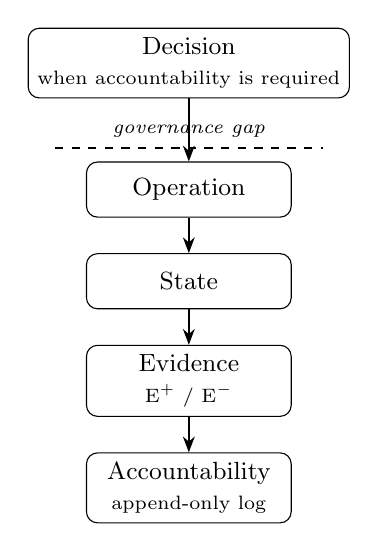
\begin{tikzpicture}[
  node distance=0.45cm,
  kbox/.style={draw, rounded corners, minimum width=2.6cm, minimum height=0.7cm, align=center, font=\small},
  arrow/.style={-Stealth, semithick}
]
  \node[kbox] (dec) {Decision\\ {\scriptsize when accountability is required}};
  \node[kbox] (op) [below=of dec, yshift=-0.35cm] {Operation};
  \node[kbox] (state) [below=of op] {State};
  \node[kbox] (ev)  [below=of state]  {Evidence\\ {\scriptsize E\textsuperscript{+} / E\textsuperscript{$-$}}};
  \node[kbox] (acc) [below=of ev]   {Accountability\\ {\scriptsize append-only log}};

  \draw[arrow] (dec)   -- (op);
  \draw[arrow] (op)    -- (state);
  \draw[arrow] (state) -- (ev);
  \draw[arrow] (ev)    -- (acc);

  % governance gap boundary
  \draw[dashed, thick] ($(op.north)+(-1.7,0.17)$) -- ($(op.north)+(1.7,0.17)$);
  \node[font=\scriptsize\itshape] at ($(op.north)+(0,0.38)$) {governance gap};
\end{tikzpicture}
}
\caption{Optional decision-binding profile. When explicit human accountability is required, the decision precedes the accountable operation. Evidence and accountability are reconstructed through the Core canonical records and referenced artifacts. The dashed line marks the proposed governance gap.}
\label{fig:kernel}
\end{figure}

\subsection{The Formal Invariant}

The central thesis of this paper's optional decision-binding profile is:

\medskip
\noindent\emph{Every accountable object within the declared profile scope should
be bound to the decision that authorized it, and that binding should be
internally auditable.}

\medskip
This is a proposed framework constraint, not a Janus Core invariant. Its utility
and domain independence require empirical evaluation.

\subsection{Implementation Surface}

The kernel is not a replacement for existing infrastructure. It introduces a governance layer that can operate over existing systems --- spreadsheets, relational databases, version control systems, AI-assisted development environments --- without requiring migration or abandonment of existing tools.

One reference implementation may use a physical file such as
\texttt{janus\_events.jsonl}. That file is not the Core ontology. A conformant
implementation preserves the conceptual separation among
\texttt{MANAGEMENT\_LOG}, \texttt{SCHEMA\_LOG}, and \texttt{AUDIT\_LOG}, even
when they share storage. E\textsuperscript{+} and E\textsuperscript{$-$} remain
classes of evidence, and \texttt{HUMAN\_DECISION} is required only when an
outcome requires explicit human accountability.

The canonical events \texttt{OMISSION\_DETECTED} and
\texttt{HUMAN\_DECISION} are defined in Janus Core~\cite{sanchez_core}. The
operational stack and a proposed evidence-based benchmark are presented in the
Framework paper~\cite{sanchez_framework}. Revised illustrative records appear
in Appendix~\ref{app:events}.

\subsection{From Pattern to Formalization}

The author's independent development process followed a recurring sequence:

A suspected structural failure is encountered in practice. An informal tool is
built to address it. The tool may then be formalized and evaluated as a
governance component. This sequence describes the author's design process; it is
not itself empirical validation.

Janus was developed independently by the author, informed in part by
longitudinal professional experience across multiple institutional and technical
contexts. No public body is represented as developer, sponsor, reviewer, or
endorser of the Core, Framework, or this paper.

The hypothesized connection among the cases is that data can carry institutional
meaning that is not captured by the operational record. The optional profile
makes accountable authorization explicit when it is required.

\subsection{Operational Interpretation (Non-Normative)}
\label{sec:opinterp}

\emph{This subsection is non-normative and describes an optional framework
profile. It adds constraints beyond Janus Core Lite and does not redefine the
Core.}

\noindent\textbf{E.1. The Kernel as a Set of Runtime Constraints}

The decision-binding profile can be implemented through three constraints:

\begin{itemize}
  \item \textbf{C1 --- Decision binding.} An operation within the declared
  profile scope that requires explicit human accountability carries a resolvable
  reference to a previously recorded \texttt{HUMAN\_DECISION}.
  \item \textbf{C2 --- Append-only correction.} Corrections are appended as new
  records or events in the corresponding canonical log. A record that declares
  supersession, correction, or voiding carries a resolvable backward reference
  to its antecedent.
  \item \textbf{C3 --- Omission evidence.} A verified absence relative to a
  versioned expectation, deterministic scope and cutoff, applicable schema, and
  reproducible observation constitutes E\textsuperscript{$-$} and may be recorded
  as \texttt{OMISSION\_DETECTED}.
\end{itemize}

These constraints define this profile and add requirements beyond the Core.

\noindent\textbf{E.2. Minimal Operational Structures}

At implementation level, the profile uses the following structures in addition
to the three canonical logs and evidence artifacts required by the Core:

\begin{itemize}
  \item \textbf{Decision record.} A Core-conformant \texttt{HUMAN\_DECISION}
  with \texttt{event\_type}, \texttt{event\_id}, \texttt{actor\_ref},
  \texttt{scope\_ref}, \texttt{object\_refs}, \texttt{occurred\_at}, and
  \texttt{recorded\_at}.
  \item \textbf{Domain record.} An identifiable record in
  \texttt{MANAGEMENT\_LOG}, interpreted under a relevant \texttt{SCHEMA\_LOG}
  schema.
  \item \textbf{Evidence artifact.} An immutable, resolvable artifact supporting
  E\textsuperscript{+} or E\textsuperscript{$-$}.
\end{itemize}

Log order alone is not normative authority. Indices, caches, and materialized
views remain implementation details and do not mutate canonical history.

\noindent\textbf{E.3. Preconditions for State Mutation}

For an accountable operation inside this optional profile, the following
preconditions hold:

\begin{enumerate}
  \item A \texttt{HUMAN\_DECISION} has already been incorporated into
  \texttt{AUDIT\_LOG} and its objects resolve.
  \item The domain operation is appended to \texttt{MANAGEMENT\_LOG} under the
  applicable schema.
  \item The implementation preserves a resolvable profile-level relationship
  between the operation and the decision without redefining Core event fields.
\end{enumerate}

Failure to meet these profile preconditions establishes nonconformance with this
profile, not automatically nonconformance with Janus Core.

\noindent\textbf{E.4. Traceability Linkage}

For an object governed by this profile, the proposed traceability path is:

\medskip
\noindent\texttt{governed object} $\rightarrow$ \texttt{domain record}
$\rightarrow$ \texttt{HUMAN\_DECISION} $\rightarrow$
\texttt{actor\_ref} + \texttt{scope\_ref}.

\medskip
If a required profile link is missing, accountability cannot be reconstructed
under the profile. Core rebuildability remains limited to governance-relevant
views and findings from its declared inputs.

\noindent\textbf{E.5. Scope of This Subsection}

This subsection does not mandate a wire format, storage backend, concurrency
model, or runtime error semantics. Concrete implementations must preserve the
Core invariants independently of this optional profile.

\section{Implications for AI-Assisted Systems}

Section~II-A proposed that AI-assisted development can amplify the hypothesized
failure through production speed, limited cross-session institutional memory,
and diffusion of attribution.

Append-only canonical logs preserve governance history. A
\texttt{HUMAN\_DECISION} can record accountable human authorization, while an
\texttt{OMISSION\_DETECTED} records E\textsuperscript{$-$} only when the Core
conditions for verified omission are met. Neither event repairs an unrecorded
past human act, and the Audit Writer may validate but does not originate a human
decision.

The governance gap is not proposed as unique to AI systems. The hypothesis is
that AI-assisted velocity can make an unrecorded authorization chain harder to
manage; operational necessity must be evaluated in each declared scope.

\section{Alignment with Existing Frameworks}

The following correspondences are interpretive mappings. They do not establish
certification or conformance with an external framework.

\subsection{NIST AI Risk Management Framework}

NIST AI RMF 1.0~\cite{nist2023} is intended for voluntary use. Janus records may
support documented roles, responsibilities, and human-oversight processes. This
paper does not claim that use of Janus establishes conformance with the AI RMF.

\subsection{W3C PROV}

Janus records can be mapped to PROV-DM~\cite{w3c_prov} only through an explicit
profile. A decision may be modeled as an activity associated with a responsible
agent and optionally a plan. PROV-DM has no native construct for the
non-occurrence of an expected activity, so E\textsuperscript{$-$} requires an
extension rather than a translation without structural change.

\subsection{ISO/IEC 42001:2023}

ISO/IEC 42001:2023~\cite{iso42001} is an AI management-system standard. No
clause-level mapping is asserted here because the licensed text was not
available among the publicly available sources cited in this paper.
Certification applies to an AI
management system and cannot be demonstrated by a technical substrate alone.

\subsection{Position}

The Janus model does not replace these frameworks. Any future mapping must name
the exact external provision, define a transformation, and provide evidence at
the scope required by that framework.

\section{Conclusion}

The central thesis of this paper is structural: systems can preserve operations
while leaving accountable human authorization outside their reconstructible
record. The retrospective practitioner cases motivate this thesis but do not
prove its prevalence or domain independence. Public documentary sources support
only the specific historical and repository facts cited; all cross-case
generalization remains academic inference.

The optional decision-binding profile addresses the proposed gap without
replacing existing infrastructure. Its profile constraint is:

\medskip
\noindent\emph{Every accountable object within the declared profile scope should
be bound to the decision that authorized it, and that binding should be
internally auditable.}

\medskip
Whether that profile is operationally necessary in a particular AI-assisted
system depends on its accountability scope and requires empirical evaluation.
Janus Core provides the underlying evidence, logging, omission, authority, and
rebuildability rules without universalizing the profile.

\clearpage
\appendices
\section{Example Governance Events}
\label{app:events}

The following synthetic examples illustrate the distinction between an evidence
artifact and canonical governance events. The identifiers and timestamps are
explicitly illustrative; they are not reconstructed historical records.

\subsection*{A.1 E\textsuperscript{+} evidence artifact}

\begin{lstlisting}[basicstyle=\ttfamily\scriptsize,breaklines=true,caption={Synthetic evidence artifact supporting E\textsuperscript{+}.},label={lst:recorded-occurrence}]
{
  "artifact_type": "recorded_observation",
  "artifact_id": "urn:example:evidence:rotation:v1",
  "recorded_at": "2026-01-01T12:00:00Z",
  "claim": "rotation observation was recorded",
  "content_digest": "sha256:example-not-a-historical-digest"
}
\end{lstlisting}

\subsection*{A.2 E\textsuperscript{$-$} recorded as \texttt{OMISSION\_DETECTED}}

\begin{lstlisting}[basicstyle=\ttfamily\scriptsize,breaklines=true,caption={Synthetic Core-conformant omission event.},label={lst:recorded-omission}]
{
  "event_type": "OMISSION_DETECTED",
  "event_id": "urn:example:audit:omission:1",
  "expectation_ref": "urn:example:schema:expectation:v1",
  "scope_ref": "urn:example:evidence:scope:v1",
  "schema_ref": "urn:example:schema:event:v1",
  "evidence_refs": ["urn:example:evidence:absence:v1"],
  "recorded_at": "2026-01-01T12:05:00Z"
}
\end{lstlisting}

\subsection*{A.3 Human authority event}

\begin{lstlisting}[basicstyle=\ttfamily\scriptsize,breaklines=true,breakatwhitespace=true,columns=fullflexible,caption={Synthetic Core-conformant human decision.},label={lst:human-authority-closure}]
{
  "event_type": "HUMAN_DECISION",
  "event_id": "urn:example:audit:decision:1",
  "actor_ref": "urn:example:actor:review-board",
  "scope_ref": "urn:example:scope:change-control:v1",
  "object_refs": ["urn:example:audit:omission:1"],
  "occurred_at": "2026-01-01T12:10:00Z",
  "recorded_at": "2026-01-01T12:11:00Z"
}
\end{lstlisting}

The evidence artifact is not a canonical governance event. The omission and
decision events are distinct append-only records; the decision neither changes
the historical omission nor constitutes E\textsuperscript{+} or
E\textsuperscript{$-$}.

\begin{thebibliography}{9}

\bibitem{sanchez_core}
M.~N. Sánchez Morales, ``JANUS: A Minimal Governance Kernel for Deterministically Reconstructible Human--AI Development Systems,'' Janus Governance Project, Argentina, 2026. DOI: 10.5281/zenodo.18974356.

\bibitem{sanchez_framework}
M.~N. Sánchez Morales, ``Janus: Evidence-Based Governance for AI-Assisted Development Systems,'' Janus Governance Project, Argentina, 2026. DOI: 10.5281/zenodo.19239183.

\bibitem{trist1951}
E.~L. Trist and K.~W. Bamforth, ``Some Social and Psychological Consequences of the Longwall Method of Coal-Getting,'' \emph{Human Relations}, vol.~4, no.~1, pp.~3--38, 1951.

\bibitem{kooi2003}
J.~Kooiman, \emph{Governing as Governance}. Sage Publications, 2003.

\bibitem{nist2023}
National Institute of Standards and Technology, ``AI Risk Management Framework (AI RMF 1.0),'' NIST, 2023. [Online]. Available: \url{https://www.nist.gov/itl/ai-risk-management-framework}

\bibitem{w3c_prov}
W3C, ``PROV-DM: The PROV Data Model,'' W3C Recommendation, 30 April 2013. [Online]. Available: \url{https://www.w3.org/TR/prov-dm/}

\bibitem{iso42001}
International Organization for Standardization, \emph{ISO/IEC 42001:2023 --- Information technology --- Artificial intelligence --- Management system}, ISO, 2023.

\bibitem{decree565}
Argentina, Decreto 565/2002, \emph{Programa Jefes de Hogar}, 3 April 2002.

\bibitem{decree1369}
Argentina, Decreto 1369/2001, dated 29 October 2001, published in the
\emph{Bolet\'in Oficial} on 31 October 2001.

\end{thebibliography}

\end{document}
